% Options for packages loaded elsewhere
% Options for packages loaded elsewhere
\PassOptionsToPackage{unicode}{hyperref}
\PassOptionsToPackage{hyphens}{url}
\PassOptionsToPackage{dvipsnames,svgnames,x11names}{xcolor}
%
\documentclass[
  12pt,
  a4paper,
  openany]{scrbook}
\usepackage{xcolor}
\usepackage[left=3cm,right=2.5cm,top=3cm,bottom=3cm]{geometry}
\usepackage{amsmath,amssymb}
\setcounter{secnumdepth}{2}
\usepackage{iftex}
\ifPDFTeX
  \usepackage[T1]{fontenc}
  \usepackage[utf8]{inputenc}
  \usepackage{textcomp} % provide euro and other symbols
\else % if luatex or xetex
  \usepackage{unicode-math} % this also loads fontspec
  \defaultfontfeatures{Scale=MatchLowercase}
  \defaultfontfeatures[\rmfamily]{Ligatures=TeX,Scale=1}
\fi
\usepackage{lmodern}
\ifPDFTeX\else
  % xetex/luatex font selection
\fi
% Use upquote if available, for straight quotes in verbatim environments
\IfFileExists{upquote.sty}{\usepackage{upquote}}{}
\IfFileExists{microtype.sty}{% use microtype if available
  \usepackage[]{microtype}
  \UseMicrotypeSet[protrusion]{basicmath} % disable protrusion for tt fonts
}{}
\makeatletter
\@ifundefined{KOMAClassName}{% if non-KOMA class
  \IfFileExists{parskip.sty}{%
    \usepackage{parskip}
  }{% else
    \setlength{\parindent}{0pt}
    \setlength{\parskip}{6pt plus 2pt minus 1pt}}
}{% if KOMA class
  \KOMAoptions{parskip=half}}
\makeatother
% Make \paragraph and \subparagraph free-standing
\makeatletter
\ifx\paragraph\undefined\else
  \let\oldparagraph\paragraph
  \renewcommand{\paragraph}{
    \@ifstar
      \xxxParagraphStar
      \xxxParagraphNoStar
  }
  \newcommand{\xxxParagraphStar}[1]{\oldparagraph*{#1}\mbox{}}
  \newcommand{\xxxParagraphNoStar}[1]{\oldparagraph{#1}\mbox{}}
\fi
\ifx\subparagraph\undefined\else
  \let\oldsubparagraph\subparagraph
  \renewcommand{\subparagraph}{
    \@ifstar
      \xxxSubParagraphStar
      \xxxSubParagraphNoStar
  }
  \newcommand{\xxxSubParagraphStar}[1]{\oldsubparagraph*{#1}\mbox{}}
  \newcommand{\xxxSubParagraphNoStar}[1]{\oldsubparagraph{#1}\mbox{}}
\fi
\makeatother

\usepackage{color}
\usepackage{fancyvrb}
\newcommand{\VerbBar}{|}
\newcommand{\VERB}{\Verb[commandchars=\\\{\}]}
\DefineVerbatimEnvironment{Highlighting}{Verbatim}{commandchars=\\\{\}}
% Add ',fontsize=\small' for more characters per line
\usepackage{framed}
\definecolor{shadecolor}{RGB}{241,243,245}
\newenvironment{Shaded}{\begin{snugshade}}{\end{snugshade}}
\newcommand{\AlertTok}[1]{\textcolor[rgb]{0.68,0.00,0.00}{#1}}
\newcommand{\AnnotationTok}[1]{\textcolor[rgb]{0.37,0.37,0.37}{#1}}
\newcommand{\AttributeTok}[1]{\textcolor[rgb]{0.40,0.45,0.13}{#1}}
\newcommand{\BaseNTok}[1]{\textcolor[rgb]{0.68,0.00,0.00}{#1}}
\newcommand{\BuiltInTok}[1]{\textcolor[rgb]{0.00,0.23,0.31}{#1}}
\newcommand{\CharTok}[1]{\textcolor[rgb]{0.13,0.47,0.30}{#1}}
\newcommand{\CommentTok}[1]{\textcolor[rgb]{0.37,0.37,0.37}{#1}}
\newcommand{\CommentVarTok}[1]{\textcolor[rgb]{0.37,0.37,0.37}{\textit{#1}}}
\newcommand{\ConstantTok}[1]{\textcolor[rgb]{0.56,0.35,0.01}{#1}}
\newcommand{\ControlFlowTok}[1]{\textcolor[rgb]{0.00,0.23,0.31}{\textbf{#1}}}
\newcommand{\DataTypeTok}[1]{\textcolor[rgb]{0.68,0.00,0.00}{#1}}
\newcommand{\DecValTok}[1]{\textcolor[rgb]{0.68,0.00,0.00}{#1}}
\newcommand{\DocumentationTok}[1]{\textcolor[rgb]{0.37,0.37,0.37}{\textit{#1}}}
\newcommand{\ErrorTok}[1]{\textcolor[rgb]{0.68,0.00,0.00}{#1}}
\newcommand{\ExtensionTok}[1]{\textcolor[rgb]{0.00,0.23,0.31}{#1}}
\newcommand{\FloatTok}[1]{\textcolor[rgb]{0.68,0.00,0.00}{#1}}
\newcommand{\FunctionTok}[1]{\textcolor[rgb]{0.28,0.35,0.67}{#1}}
\newcommand{\ImportTok}[1]{\textcolor[rgb]{0.00,0.46,0.62}{#1}}
\newcommand{\InformationTok}[1]{\textcolor[rgb]{0.37,0.37,0.37}{#1}}
\newcommand{\KeywordTok}[1]{\textcolor[rgb]{0.00,0.23,0.31}{\textbf{#1}}}
\newcommand{\NormalTok}[1]{\textcolor[rgb]{0.00,0.23,0.31}{#1}}
\newcommand{\OperatorTok}[1]{\textcolor[rgb]{0.37,0.37,0.37}{#1}}
\newcommand{\OtherTok}[1]{\textcolor[rgb]{0.00,0.23,0.31}{#1}}
\newcommand{\PreprocessorTok}[1]{\textcolor[rgb]{0.68,0.00,0.00}{#1}}
\newcommand{\RegionMarkerTok}[1]{\textcolor[rgb]{0.00,0.23,0.31}{#1}}
\newcommand{\SpecialCharTok}[1]{\textcolor[rgb]{0.37,0.37,0.37}{#1}}
\newcommand{\SpecialStringTok}[1]{\textcolor[rgb]{0.13,0.47,0.30}{#1}}
\newcommand{\StringTok}[1]{\textcolor[rgb]{0.13,0.47,0.30}{#1}}
\newcommand{\VariableTok}[1]{\textcolor[rgb]{0.07,0.07,0.07}{#1}}
\newcommand{\VerbatimStringTok}[1]{\textcolor[rgb]{0.13,0.47,0.30}{#1}}
\newcommand{\WarningTok}[1]{\textcolor[rgb]{0.37,0.37,0.37}{\textit{#1}}}

\usepackage{longtable,booktabs,array}
\usepackage{calc} % for calculating minipage widths
% Correct order of tables after \paragraph or \subparagraph
\usepackage{etoolbox}
\makeatletter
\patchcmd\longtable{\par}{\if@noskipsec\mbox{}\fi\par}{}{}
\makeatother
% Allow footnotes in longtable head/foot
\IfFileExists{footnotehyper.sty}{\usepackage{footnotehyper}}{\usepackage{footnote}}
\makesavenoteenv{longtable}
\usepackage{graphicx}
\makeatletter
\newsavebox\pandoc@box
\newcommand*\pandocbounded[1]{% scales image to fit in text height/width
  \sbox\pandoc@box{#1}%
  \Gscale@div\@tempa{\textheight}{\dimexpr\ht\pandoc@box+\dp\pandoc@box\relax}%
  \Gscale@div\@tempb{\linewidth}{\wd\pandoc@box}%
  \ifdim\@tempb\p@<\@tempa\p@\let\@tempa\@tempb\fi% select the smaller of both
  \ifdim\@tempa\p@<\p@\scalebox{\@tempa}{\usebox\pandoc@box}%
  \else\usebox{\pandoc@box}%
  \fi%
}
% Set default figure placement to htbp
\def\fps@figure{htbp}
\makeatother


% definitions for citeproc citations
\NewDocumentCommand\citeproctext{}{}
\NewDocumentCommand\citeproc{mm}{%
  \begingroup\def\citeproctext{#2}\cite{#1}\endgroup}
\makeatletter
 % allow citations to break across lines
 \let\@cite@ofmt\@firstofone
 % avoid brackets around text for \cite:
 \def\@biblabel#1{}
 \def\@cite#1#2{{#1\if@tempswa , #2\fi}}
\makeatother
\newlength{\cslhangindent}
\setlength{\cslhangindent}{1.5em}
\newlength{\csllabelwidth}
\setlength{\csllabelwidth}{3em}
\newenvironment{CSLReferences}[2] % #1 hanging-indent, #2 entry-spacing
 {\begin{list}{}{%
  \setlength{\itemindent}{0pt}
  \setlength{\leftmargin}{0pt}
  \setlength{\parsep}{0pt}
  % turn on hanging indent if param 1 is 1
  \ifodd #1
   \setlength{\leftmargin}{\cslhangindent}
   \setlength{\itemindent}{-1\cslhangindent}
  \fi
  % set entry spacing
  \setlength{\itemsep}{#2\baselineskip}}}
 {\end{list}}
\usepackage{calc}
\newcommand{\CSLBlock}[1]{\hfill\break\parbox[t]{\linewidth}{\strut\ignorespaces#1\strut}}
\newcommand{\CSLLeftMargin}[1]{\parbox[t]{\csllabelwidth}{\strut#1\strut}}
\newcommand{\CSLRightInline}[1]{\parbox[t]{\linewidth - \csllabelwidth}{\strut#1\strut}}
\newcommand{\CSLIndent}[1]{\hspace{\cslhangindent}#1}



\setlength{\emergencystretch}{3em} % prevent overfull lines

\providecommand{\tightlist}{%
  \setlength{\itemsep}{0pt}\setlength{\parskip}{0pt}}



 


\usepackage{subcaption}
\captionsetup[subfigure]{list=false}
% \AddToHook{cmd/section/before}{\clearpage}  % new page for each section for articles

% make all sectioning heads (chapter/section/subsection/…) serif for srcbook
\setkomafont{disposition}{\normalfont\bfseries\rmfamily}

\usepackage{hyperref}
\usepackage[nameinlink, capitalise, noabbrev]{cleveref} % \cref{_label_} to link the label and section number 

\usepackage{threeparttable}
\usepackage{adjustbox} 
\usepackage{amsmath,amssymb}
\usepackage{unicode-math}
\setmathfont{Latin Modern Math}
\usepackage{booktabs, caption, longtable, colortbl, array}
\usepackage{threeparttable}
\usepackage{enumitem}
% \usepackage{float}  % for \begin{table}[h] ? check
% \setlist[description]{nosep,style=multiline,leftmargin=3.5cm,font=\normalfont\textsf}

\PassOptionsToPackage{list=true}{subcaption}    % fix fig-scap in list of figs. 

%% To prevent hyphenation
%\tolerance=1
%\emergencystretch=\maxdimen
%\hyphenpenalty=10000
%\hbadness=10000
%% END hyphenation

\usepackage{geometry}
\usepackage[T1]{fontenc} 
\usepackage[utf8]{inputenc}
\usepackage[ngerman,english]{babel}
\usepackage{setspace}
\usepackage{titling}
\usepackage{parskip}
% \usepackage{helvet}
% \renewcommand{\familydefault}{\sfdefault} % Use sans-serif
\renewcommand{\bfdefault}{b}      % <-- key: make \textbf use 'b'
\usepackage{graphicx}
\usepackage{xcolor}
\usepackage[font=footnotesize,labelfont={bf, footnotesize}]{caption}
\captionsetup{
  format=plain,                % no hanging indent
  justification=justified     % full-width text
}

\setlength{\droptitle}{-5em}
\onehalfspacing
\makeatletter
\@ifpackageloaded{bookmark}{}{\usepackage{bookmark}}
\makeatother
\makeatletter
\@ifpackageloaded{caption}{}{\usepackage{caption}}
\AtBeginDocument{%
\ifdefined\contentsname
  \renewcommand*\contentsname{Table of contents}
\else
  \newcommand\contentsname{Table of contents}
\fi
\ifdefined\listfigurename
  \renewcommand*\listfigurename{List of Figures}
\else
  \newcommand\listfigurename{List of Figures}
\fi
\ifdefined\listtablename
  \renewcommand*\listtablename{List of Tables}
\else
  \newcommand\listtablename{List of Tables}
\fi
\ifdefined\figurename
  \renewcommand*\figurename{Figure}
\else
  \newcommand\figurename{Figure}
\fi
\ifdefined\tablename
  \renewcommand*\tablename{Table}
\else
  \newcommand\tablename{Table}
\fi
}
\@ifpackageloaded{float}{}{\usepackage{float}}
\floatstyle{ruled}
\@ifundefined{c@chapter}{\newfloat{codelisting}{h}{lop}}{\newfloat{codelisting}{h}{lop}[chapter]}
\floatname{codelisting}{Listing}
\newcommand*\listoflistings{\listof{codelisting}{List of Listings}}
\makeatother
\makeatletter
\makeatother
\makeatletter
\@ifpackageloaded{caption}{}{\usepackage{caption}}
\@ifpackageloaded{subcaption}{}{\usepackage{subcaption}}
\makeatother
\usepackage{bookmark}
\IfFileExists{xurl.sty}{\usepackage{xurl}}{} % add URL line breaks if available
\urlstyle{same}
\hypersetup{
  pdftitle={Edit: Master Thesis Title},
  pdfauthor={Jorge Eduardo Frías Navarrete},
  colorlinks=true,
  linkcolor={blue},
  filecolor={Maroon},
  citecolor={Blue},
  urlcolor={Blue},
  pdfcreator={LaTeX via pandoc}}


\title{Edit: Master Thesis Title}
\author{Jorge Eduardo Frías Navarrete}
\date{August 18, 2025}
\begin{document}
\frontmatter

%------------------------------------------------
% Declaring new geometry for the title page only.
\newgeometry{left=2cm,right=2cm,top=2cm,bottom=2cm}
%------------------------------------------------

\thispagestyle{empty}
\begin{figure}[h!]
    \raggedleft
    
\includegraphics[scale=0.9]{pictures/WULogo.png}
\end{figure}

\vspace{1em}

\begin{center}
    \large Master Thesis \\
    \vspace{1cm}

    \textbf{\huge Edit: Master Thesis Title} \\
    \vspace{0.5cm}

        \LARGE Jorge Eduardo \textsc{Frías Navarrete} \\
    \vspace{0.5cm}
    %\Large Jorge Eduardo Frías Navarrete \\
        \vspace{2cm}
    
    \normalsize Submitted in partial fulfillment of the requirement for the degree of: \\
    \LARGE Master of Science \\
\vspace{2cm}

\normalsize
    \begin{tabular}{ll}
        Student ID: & 012329686 \\
        Degree programme: & Quantitative Finance \\
        %University: & Vienna University of Economics and Business \\
        Supervisor: & Univ.Prof. David \textsc{Preinerstorfer}, Ph.D. \\
        Date of Submission: & August 18, 2025
    \end{tabular}
    \vspace{2cm}
    
    \textit{
    %\begin{tabular}{l}
      Department of Finance, Accounting and Statistics. \\
      Vienna University of Economics and Business. \\
      Welthandelsplatz 1, 1020 Vienna, Austria.
    %\end{tabular}
    }

\end{center}

%-----------------------------------------------
\restoregeometry
%-----------------------------------------------


% \begin{center}
%   \normalfont\bfseries Abstract
% \end{center}
% 
% \begin{center}
%   \begin{minipage}{0.8\textwidth}
%     \small
%     Here goes my abstract in Quarto. Random text: 
%     If you have a book with several pages in a section or subsection, it is often convenient to offer the user the ability to navigate to the next page (or previous page) at the bottom of the page that they’ve just finished reading. You can enable this using.
%   \end{minipage}
% \end{center}


% 
% \addchap*{Abstract}
% 
% Here goes my abstract text. Here goes my abstract text. Here goes my abstract text.
% Lorem ipsum dolor sit amet, consectetur adipiscing elit. Suspendisse eu dolor luctus, rhoncus leo in, commodo turpis. Aenean sed enim in sem euismod porta. Vivamus tempor lorem nec eros rhoncus, eu hendrerit libero tincidunt. Class aptent taciti sociosqu ad litora torquent per conubia nostra, per inceptos himenaeos. Pellentesque habitant morbi tristique senectus et netus et malesuada fames ac turpis egestas. Lorem ipsum dolor sit amet, consectetur adipiscing elit. Quisque dapibus turpis quis nibh molestie dapibus. Aliquam erat volutpat. Integer et odio nec mauris sollicitudin mattis. 
% 

\let\mainmatterreal\mainmatter
\let\mainmatter\relax
% Open right for these sections: blank page to make section start on the right side. 
\KOMAoptions{open=right}  

\renewcommand*\contentsname{Table of contents}
% Set toc black if tcocolor = black
% % \hypersetup{linkcolor=}
% \setcounter{tocdepth}{1}
\renewcommand*\listfigurename{List of figures}
\renewcommand*\listtablename{List of tables}

% Open right for these sections: blank page to make section start on the right side. 
\KOMAoptions{open=right}  
\mainmatter
\bookmarksetup{startatroot}

\chapter*{Acknowledgements}\label{acknowledgements}

\markboth{Acknowledgements}{Acknowledgements}

Here write acknowledgements.

\bookmarksetup{startatroot}

\chapter*{Abstract}\label{abstract}

\markboth{Abstract}{Abstract}

Here goes my abstract text. Here goes my abstract text. Here goes my
abstract text. Lorem ipsum dolor sit amet, consectetur adipiscing elit.
Suspendisse eu dolor luctus, rhoncus leo in, commodo turpis. Aenean sed
enim in sem euismod porta. Vivamus tempor lorem nec eros rhoncus, eu
hendrerit libero tincidunt. Class aptent taciti sociosqu ad litora
torquent per conubia nostra, per inceptos himenaeos. Pellentesque
habitant morbi tristique senectus et netus et malesuada fames ac turpis
egestas. Lorem ipsum dolor sit amet, consectetur adipiscing elit.
Quisque dapibus turpis quis nibh molestie dapibus. Aliquam erat
volutpat. Integer et odio nec mauris sollicitudin mattis.

% make toc black (for some reason, toccolor does not work)
{\hypersetup{linkcolor=black}
\tableofcontents 

% lof and lot on the same page
\listoffigures
\begingroup
\let\clearpage\relax
\listoftables
\endgroup
}

% Return to arabic numbering after this section
\let\mainmatter\mainmatterreal
\mainmatter

% Return to open any (no blank pages)
\KOMAoptions{open=any}    % restore your global default

\bookmarksetup{startatroot}

\chapter{Introduction}\label{introduction}

Mirar Liu et al (y el otro paper similar) donde habla de las
criptomonedas, e inspirarnos de ahi. Quiza la otra tesis en esto
tambien.

Empezar con una introduccion de criptomonedas, del mercado, de la gran
volatilidad, grandes retornos. Mencionar coin Market cap, la
capitalizacion del mercado total de criptomonedas.

Mencionar articulos o reportes donde mencionen la importancia de este
mercado, cuantas personas en promedio tienen criptos en su portafolio.
Mencionar sucesos recientes importantes, como la introduccion de
criptomonedas en algunos exchanges, de futuros en CME, de indices en
XXX, del boom en la crisis de COVID (ver Mercik, donde menciona sucesos
importantes).

mencionar a Ross, que comprobo la estructura lineal de los factores: --
Esto quiza en introduccion

** Ejemplo de frase See (\citeproc{ref-knuth84}{\textbf{knuth84?}}) for
additional discussion of literate programming.**

\begin{Shaded}
\begin{Highlighting}[]
\DecValTok{1} \SpecialCharTok{+} \DecValTok{1}
\end{Highlighting}
\end{Shaded}

\begin{verbatim}
[1] 2
\end{verbatim}

\bookmarksetup{startatroot}

\chapter{Methodology}\label{methodology}

The Instrumented Principal Component Analysis (IPCA) model was
introduced in the seminal work of Kelly et al.
(\citeproc{ref-kellyCharacteristicsAre2019}{2019},
\citeproc{ref-kellyInstrumentedPrincipal2020}{2020}). The main model
used in this thesis is the IPCA with different \(K\) number of factors

Explicar la metodologia de IPCA. Si hay tiempo, entonces explicar
tambien como funciona el RPCA de Chen and Roussanov. Explicar las R2 (en
lugra de R2, entonces poner Total score y predictive score), mencionar
como pie de pagina que son las medidas definidas por Kelly et al.
(\citeproc{ref-kellyCharacteristicsAre2019}{2019}).

Explicar los bootstrap para medir la significancia cada caracteristica,
y quiza mencionar tambi'en brevemente los characteristic managed
portfolios, en que consisten y como se emplean (quiza tomar inspiracion
de Kelly, Bianchi, o creo que puede ser mejor en Liu et al.)

\section{Instrumented Principal Component
Analysis}\label{instrumented-principal-component-analysis}

\bookmarksetup{startatroot}

\chapter{Data}\label{data}

In this section, I introduce the cryptocurrency data used in this
thesis, the series of filters applied to clean and prepare the dataset,
and the summary statistics of the cryptocurrency excess returns. In
addition, I show the set of asset-specific characteristics constructed
from the cryptocurrency market data, which are used as instruments for
latent factor exposures in the IPCA model. Appendix
\ref{sec-app_characteristics} provides a detailed description of the
characteristics used in the empirical analysis.

\textbf{{[}++++ ADD SMALL INTRO ABOVE OF RIK FACTORS CREATED ++++{]}}

The data extraction and pre-processing are primarily conducted in R
4.5.1 (\citeproc{ref-base}{R Core Team, 2025}), using, among other
packages\footnote{See Appendix~\ref{sec-software} for the full list of
  software used in the empirical study.}, the \texttt{tidyverse} (v.
2.0.0; \citeproc{ref-tidyverse}{Wickham et al., 2019}). Additional
cleaning steps and visualizations are performed in Python 3.13.5
(\citeproc{ref-python}{Python Software Foundation, 2025}). The full
reproducible code is available in Appendix \ref{sec-app_material}.

\section{Data extraction and sample
construction}\label{data-extraction-and-sample-construction}

I collect daily cryptocurrency data on open, high, close, and low (OHCL)
prices, 24-hour volume, and market capitalization (calculated as the
cryptocurrency's USD price multiplied by its circulating supply) from
\href{https://coincodex.com/}{CoinCodex}, a website-data provider that
gathers and aggregates data from more than 400 exchanges. I extract the
data, all expressed in US dollars, using the CoinCodex API as follows:

\begin{enumerate}
\def\labelenumi{\arabic{enumi}.}
\item
  I retrieve the list of all available cryptocurrencies and extract each
  cryptocurrency shortname, also referred to as the ``slug''. At the
  time of writing, there are 14,907 unique cryptocurrency shortnames
  listed in the API.
\item
  Using the slug, I construct an URL for each cryptocurrency to obtain
  the metadata from the API. I parse the JSON API response into a
  dataframe and extract the OHCL prices, volume, and market
  capitalization daily data. I exclude those observations with non-zero
  or missing values in any of these fields.
\end{enumerate}

Out of the 14,907 cryptocurrencies listed, only 7,272 entries contained
available data. Next, following the methodology of Bianchi \& Babiak
(\citeproc{ref-bianchiMispricingRiskCompensation2021}{2021}) and Mercik
et al.
(\citeproc{ref-mercikCrosssectionalInteractionsCryptocurrency2025}{2025}),
I apply a series of cleaning and filtering steps in order to remove
possible innacuracies in the dataset:

\begin{enumerate}
\def\labelenumi{\arabic{enumi}.}
\item
  Non-positive and missing values. As mentioned earlier, I remove
  observations where prices, volume, or market capitalization were
  non-positive or missing.
\item
  Small cryptocurrencies. Similar to Liu et al.
  (\citeproc{ref-liuCommonRisk2022}{2022}), I screen out small
  cryptocurrencies and consider only those with a market capitalization
  greater than one million USD. Therefore, I exclude observations for
  coins whose market capitalization falls below this minimum threshold,
  which allows for the possibility that a coin may become ``small''
  after a certain period or event.
\item
  Cryptocurrency type. Based on the cryptocurrency classification from
  \href{https://coinmarketcap.com/cryptocurrency-category/}{CoinMarketCap}
  and CoinCodex, I exclude:

  \begin{itemize}
  \item
    stablecoins. I include (i) centralized stablecoins, which are backed
    and pegged to fiat currency or physical assets by a third party,
    such as Tether (USDT), USD Coin (USDC), and Euro Coin (EURC), and
    (ii) algorithmically stabilized stablecoins, which use algorithms to
    adjust the circulating supply in response to changes in demand to
    maintain a stable value with the underlying asset, such as DAI and
    AMPL (FSB,
    \citeproc{ref-financialstabilityboardAddressingRegulatory2020}{2020}).
  \item
    wrapped cryptocurrency tokens, which mirror the value of another
    cryptocurrency from a different blockchain, e.g., Wrapped Bitcoin
    (wBTC) or Wrapped Ethereum (wETH)
    (\citeproc{ref-coinbaseWhatWrapped}{Coinbase, n.d.}).
  \item
    cryptocurrencies backed by or pegged to gold or precious metals,
    including Pax Gold (PAXG) or XAGx Silver Token (XAGX).
  \end{itemize}
\item
  Erroneous trading volume. To filter out cryptocurrencies with ``fake''
  or ``erroneous'' trading volume, I calculate the daily
  volume-to-market-capitalization ratio for each token and exclude
  observations where the ratio exceeds 1.
\item
  Extreme returns. To minimize the influence of extreme values in my
  results, I winsorize daily cryptocurrency returns to lie within the
  range of -90\% to 500\%.
\item
  Time period. Even though cryptocurrency data are available since 2014,
  I use data from June 1, 2018 for the empirical analysis due to the low
  amount of coins available before this date (see
  Figure~\ref{fig-numcoins}).
\item
  Minimum observations. In order to maintain practical relevance, I keep
  cryptocurrencies that have at least 365 consecutive daily observations
  and those with at least 730 observations in the complete panel of coin
  characteristics (see Section~\ref{sec-characteristics}), which is
  equivalent to 2 years of historical data. Therefore, I exclude very
  short-lived coins, but retain failed coins with this relatively large
  number of observations, which help to lessen the so called
  ``survivorship biais''.
\end{enumerate}

\begin{figure}[h]

\centering{

\centering{

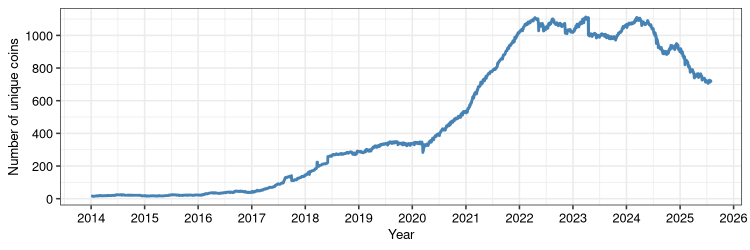
\includegraphics[width=0.8\linewidth,height=\textheight,keepaspectratio]{pictures/timeseries_daily_coins.png}

}

\subcaption{\label{fig-sub1}}

\centering{

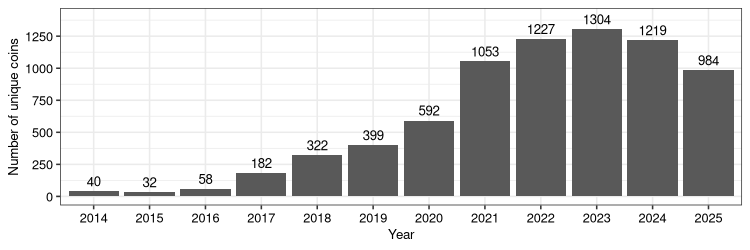
\includegraphics[width=0.8\linewidth,height=\textheight,keepaspectratio]{pictures/coins_per_year.png}

}

\subcaption{\label{fig-sub2}}

}

\caption[Number of cryptocurrencies over
time]{\label{fig-numcoins}\textbf{Number of cryptocurrencies over time.}
Panel A shows the daily time series of the number of unique
cryptocurrencies. Panel B displays the number of unique cryptocurrencies
recorded each year. Both panels correspond to the dataset after applying
the filtering steps (1) to (5), covering the period from January 1,
2014, to July 31, 2025, and including 1,416 unique cryptocurrencies.
Note that coins may enter or exit the market over time.}

\end{figure}%

\section{Sample overview}\label{sample-overview}

After applying all the filters, the resulting sample consists of 973
unique cryptocurrencies and 1,478,936 observations from June 1, 2018, to
July 31, 2025, where a day starts at 00:00:00 UTC. It is important to
mention that the number of cryptocurrencies fluctuates over the entire
period, which results in an unbalanced panel of data.

\begin{table}[t]
\centering
\caption[Summary statistics of daily excess returns]{\textbf{Summary statistics of daily excess returns.} The table reports summary statistics of daily excess returns for the filtered sample, the top 100 cryptocurrencies ranked by market capitalization, and for Bitcoin, Ethereum, and Ripple individually. Reported statistics include the number of daily observations, the number of unique coins over the sample period, the mean and standard deviation of returns, and the 10th percentile, lower quartile, median, upper quartile, and 90th percentile of the distribution of the returns. The sample period is from June 1, 2018, to July 31, 2025.}
\label{tbl-overview}
\begin{adjustbox}{max width=\textwidth}
\begin{threeparttable}
\begin{tabular}{lccccccccc}
\toprule
 & No. Obs & Unique coins & Mean & Std & P10 & P25 & P50 & P75 & P90 \\
\midrule
Sample & 1,478,936 & 973 & -2.70\% & 12.49\% & -10.18\% & -6.65\% & -3.70\% & 0.02\% & 4.69\% \\
Top 100 & 176,400 & 100 & -2.94\% & 7.28\% & -9.20\% & -6.32\% & -3.56\% & -0.16\% & 3.67\% \\
Top 10\tnote{1} & 24,747 & 10 & -2.35\% & 6.14\% & -7.80\% & -5.44\% & -2.87\% & 0.22\% & 3.55\% \\
Bitcoin & 2,618 &  & -2.40\% & 3.92\% & -6.60\% & -4.96\% & -2.58\% & -0.20\% & 2.26\% \\
Ethereum & 2,611 &  & -2.40\% & 4.85\% & -7.46\% & -5.27\% & -2.83\% & 0.27\% & 3.48\% \\
Ripple & 2,540 &  & -2.41\% & 5.70\% & -7.65\% & -5.43\% & -2.77\% & -0.00\% & 2.87\% \\
\bottomrule
\end{tabular}
\begin{tablenotes}\footnotesize
\item[1] As of July 31, 2025, the top 10 cryptocurrencies are Bitcoin, Ethereum, Ripple, Binance Coin, Solana, Dogecoin, Tron, Cardano, Stellar, and Chainlink.
\end{tablenotes}
\end{threeparttable}
\end{adjustbox}
\end{table}

\section{Characteristic construction and
description}\label{sec-characteristics}

Following Kelly et al.
(\citeproc{ref-kellyCharacteristicsAre2019}{2019}), I cross-sectionally
transform the instrument variables period-by-period in the following
manner: first,

This is more related to factor construction.

Organize week in the following way: the first seven days of the year
forms the first week, and the first 51 weeks of the year consists of 7
days each. The 52th week of the year consists of the last eight days
and, in case of a leap year (as 2016, 2020, and 2024), of nine days.

Following Liu et al. (\citeproc{ref-liuCommonRisk2022}{2022}), I
construct a daily cryptocurrency market return as the value-weighted
average return of all the cryptocurrencies in the sample. For
cryptocurrencies \(i = 1, ..., N\), the daily market return at time
\(t\) is computed as:

\[
r_t^M = \frac{\sum_{i=1}^N r_{it} \cdot marketcap_{it}}
             {\sum_{i=1}^N marketcap_{it} }
\]

The cryptocurrency market excess return is constructed as the difference
between the cryptocurrency market return and the risk-free rate. To
proxy the risk-free rate, I used the (daily) 1-month Treasury bill rate
from the FRED.

Write this in the following section of ``Empirical application'' or This
is for the model: 7. (Still undecisive) Minimum cross-section. Following
the criterion by Kelly, I Convert variables in the -0.5 - 0.5 range

The sample period ranges from January 1st, 2014, to May 31st, 2025.

\bookmarksetup{startatroot}

\chapter{Results}\label{results}

Implemented in python, based on the IPCA python code of Seth Pruitt
\footnote{See https://sethpruitt.net/research/.} and the \texttt{ipca}
python package of Buechner \& Bybee (\citeproc{ref-ipca}{2019})
\footnote{See https://bkelly-lab.github.io/ipca/.}.

\textbf{Important}: mention the shift of characteristics: the
conditional APT of Kelly, Pruitt, Su (JFE 2019) says that the
characteristics known at Date=d-1 determine the exposures associated
with the returns realized at Date=d; hence, here we should have shifted
the characteristics in Z relative to the returns in R

This is a template of the table of the results of the IPCA model. I need
to add a caption to the table. Here I reference Table
\ref{tbl-ipca_results}.

\begin{table}
\centering
\small
%\fontsize{9.0pt}{10.8pt}\selectfont
\caption[Results of IPCA regression]%
{%
\textbf{Results of IPCA regression.}
Model Performance. Panel A and B report total and predictive $R^2$ in percent for the restricted ($\Gamma_\alpha = 0$) and unrestricted ($\Gamma_\alpha \neq 0$) IPCA model for $K$ number of factors on daily and weekly data, respectively. Panel C reports the corresponding total and predictive $R^2$ for a simple PCA model on weekly data.
}
\label{tbl-ipca_results}
\begin{tabular}{lcccc}
\toprule
 &  & \multicolumn{3}{c}{K } \\
\cmidrule(lr){3-5}
 &  & \(K = 3\) & \(K = 5\) & \(K = 8\) \\
\midrule\addlinespace[2.5pt]
\multicolumn{5}{l}{Panel C: PCA on weekly data} \\[2.5pt]
\midrule\addlinespace[2.5pt]
\(R^{2}_{\text{Total}}\) &  & 0.0000 & 0.0000 & 0.0000 \\
\(R^{2}_{\text{Predictive}}\) &  & 0.0000 & 0.0000 & 0.0000 \\
\midrule\addlinespace[2.5pt]
\multicolumn{5}{l}{Panel B: IPCA on weekly data} \\[2.5pt]
\midrule\addlinespace[2.5pt]
\(R^{2}_{\text{Total}}\) & \(\Gamma_{\alpha} = 0\) & 0.2625 & 0.2817 & 0.2934 \\
 & \(\Gamma_{\alpha} \neq 0\) & 0.2661 & 0.2826 & 0.2937 \\
\(R^{2}_{\text{Predictive}}\) & \(\Gamma_{\alpha} = 0\) & 0.1725 & 0.1551 & 0.1511 \\
 & \(\Gamma_{\alpha} \neq 0\) & 0.1719 & 0.1584 & 0.1554 \\
\midrule\addlinespace[2.5pt]
\multicolumn{5}{l}{Panel A: IPCA on daily data} \\[2.5pt]
\midrule\addlinespace[2.5pt]
\(R^{2}_{\text{Total}}\) & \(\Gamma_{\alpha} = 0\) & 0.2301 & 0.2509 & 0.2681 \\
 & \(\Gamma_{\alpha} \neq 0\) & 0.2322 & 0.2524 & 0.2690 \\
\(R^{2}_{\text{Predictive}}\) & \(\Gamma_{\alpha} = 0\) & -0.3904 & -0.4082 & -0.4169 \\
 & \(\Gamma_{\alpha} \neq 0\) & -0.3857 & -0.4055 & -0.4156 \\
\bottomrule
\end{tabular}
\end{table}

Some test for quarto and latex

Quarto: 1. Sees the caption line after the table. 2. Wraps the
\texttt{tabular} inside a LaTeX \texttt{table} environment. 3. Adds
\texttt{\textbackslash{}caption\{Some\ letters\ with\ LaTeX\}} and
\texttt{\textbackslash{}label\{tbl-letters\}} automatically. 4. Gives it
a table number and puts it in the List of Tables.

\begin{center}\rule{0.5\linewidth}{0.5pt}\end{center}

\textbf{Inline LaTeX way inside Quarto}\\
Here we see the summary statistics in Table \ref{tbl-letters}.

\begin{table}

\caption{\label{tbl-letters}Some letters with LaTeX}

\centering{

\centering

\begin{tabular}{lll}
A & B & C \\
D & E & F \\
\end{tabular}

}

\end{table}%

\bookmarksetup{startatroot}

\chapter{Conclusion}\label{conclusion}

\bookmarksetup{startatroot}

\chapter*{References}\label{references}
\addcontentsline{toc}{chapter}{References}

\markboth{References}{References}

\phantomsection\label{refs}
\begin{CSLReferences}{1}{0}
\bibitem[\citeproctext]{ref-Quarto_2025}
Allaire, J. J., Teague, C., Scheidegger, C., Xie, Y., Dervieux, C., \&
Woodhull, G. (2025). \emph{{Quarto}} (Version 1.7) {[}Computer
software{]}. \url{https://doi.org/10.5281/zenodo.5960048}

\bibitem[\citeproctext]{ref-bidask}
Ardia, D., Guidotti, E., \& Kroencke, T. A. (2024). Efficient estimation
of bid--ask spreads from open, high, low, and close prices.
\emph{Journal of Financial Economics}, \emph{161}, 103916.
\url{https://doi.org/10.1016/j.jfineco.2024.103916}

\bibitem[\citeproctext]{ref-bianchiMispricingRiskCompensation2021}
Bianchi, D., \& Babiak, M. (2021). \emph{Mispricing and Risk
Compensation in Cryptocurrency Returns} (SSRN Scholarly Paper 3935934).
Social Science Research Network.
\url{https://doi.org/10.2139/ssrn.3935934}

\bibitem[\citeproctext]{ref-ipca}
Buechner, M., \& Bybee, L. (2019). \emph{{ipca}: Instrumented principal
components analysis} {[}Computer software{]}.
\url{https://github.com/bkelly-lab/ipca}

\bibitem[\citeproctext]{ref-coinbaseWhatWrapped}
Coinbase. (n.d.). \emph{What is wrapped crypto?} Retrieved August 6,
2025, from
\url{https://www.coinbase.com/learn/your-crypto/what-is-wrapped-crypto}

\bibitem[\citeproctext]{ref-financialstabilityboardAddressingRegulatory2020}
Financial Stability Board. (2020). \emph{Addressing the regulatory,
supervisory and oversight challenges raised by {``global stablecoin''}
arrangements: Consultative document}.
\url{https://www.fsb.org/2020/04/addressing-the-regulatory-supervisory-and-oversight-challenges-raised-by-global-stablecoin-arrangements-consultative-document/}

\bibitem[\citeproctext]{ref-harris2020array}
Harris, C. R., Millman, K. J., Walt, S. J. van der, Gommers, R.,
Virtanen, P., Cournapeau, D., Wieser, E., Taylor, J., Berg, S., Smith,
N. J., Kern, R., Picus, M., Hoyer, S., Kerkwijk, M. H. van, Brett, M.,
Haldane, A., Río, J. F. del, Wiebe, M., Peterson, P., \ldots{} Oliphant,
T. E. (2020). Array programming with {NumPy}. \emph{Nature},
\emph{585}(7825), 357--362.
\url{https://doi.org/10.1038/s41586-020-2649-2}

\bibitem[\citeproctext]{ref-Hunter:2007}
Hunter, J. D. (2007). Matplotlib: A 2D graphics environment.
\emph{Computing in Science \& Engineering}, \emph{9}(3), 90--95.
\url{https://doi.org/10.1109/MCSE.2007.55}

\bibitem[\citeproctext]{ref-kellyCharacteristicsAre2019}
Kelly, B. T., Pruitt, S., \& Su, Y. (2019). Characteristics are
covariances: A unified model of risk and return. \emph{Journal of
Financial Economics}, \emph{134}(3), 501--524.
\url{https://doi.org/10.1016/j.jfineco.2019.05.001}

\bibitem[\citeproctext]{ref-kellyInstrumentedPrincipal2020}
Kelly, B. T., Pruitt, S., \& Su, Y. (2020). \emph{Instrumented Principal
Component Analysis} (SSRN Scholarly Paper 2983919). Social Science
Research Network. \url{https://doi.org/10.2139/ssrn.2983919}

\bibitem[\citeproctext]{ref-moments}
Komsta, L., \& Novomestky, F. (2022). \emph{{moments}: Moments,
cumulants, skewness, kurtosis and related tests}.
\url{https://doi.org/10.32614/CRAN.package.moments}

\bibitem[\citeproctext]{ref-liuCommonRisk2022}
Liu, Y., Tsyvinski, A., \& Wu, X. (2022). Common Risk Factors in
Cryptocurrency. \emph{The Journal of Finance}, \emph{77}(2), 1133--1177.
\url{https://doi.org/10.1111/jofi.13119}

\bibitem[\citeproctext]{ref-mercikCrosssectionalInteractionsCryptocurrency2025}
Mercik, A., Będowska-Sójka, B., Karim, S., \& Zaremba, A. (2025).
Cross-sectional interactions in cryptocurrency returns.
\emph{International Review of Financial Analysis}, \emph{97}, 103809.
\url{https://doi.org/10.1016/j.irfa.2024.103809}

\bibitem[\citeproctext]{ref-moskowitzTimeSeriesMomentum2012}
Moskowitz, T. J., Ooi, Y. H., \& Pedersen, L. H. (2012). Time series
momentum. \emph{Journal of Financial Economics}, \emph{104}(2),
228--250. \url{https://doi.org/10.1016/j.jfineco.2011.11.003}

\bibitem[\citeproctext]{ref-PerformanceAnalytics}
Peterson, B. G., \& Carl, P. (2024). \emph{{PerformanceAnalytics}:
Econometric tools for performance and risk analysis}.
\url{https://doi.org/10.32614/CRAN.package.PerformanceAnalytics}

\bibitem[\citeproctext]{ref-rstudio}
Posit team. (2025). \emph{{RStudio}: Integrated development environment
for r}. Posit Software, PBC. \url{http://www.posit.co/}

\bibitem[\citeproctext]{ref-python}
Python Software Foundation. (2025). \emph{Python programming language}
(Version 3.13.5) {[}Computer software{]}. \url{https://www.python.org/}

\bibitem[\citeproctext]{ref-base}
R Core Team. (2025). \emph{R: A language and environment for statistical
computing}. R Foundation for Statistical Computing.
\url{https://www.R-project.org/}

\bibitem[\citeproctext]{ref-quantmod}
Ryan, J. A., \& Ulrich, J. M. (2025). \emph{{quantmod}: Quantitative
financial modelling framework}.
\url{https://doi.org/10.32614/CRAN.package.quantmod}

\bibitem[\citeproctext]{ref-pcaMethods}
Stacklies, W., Redestig, H., Scholz, M., Walther, D., \& Selbig, J.
(2007). pcaMethods -- a bioconductor package providing PCA methods for
incomplete data. \emph{Bioinformatics}, \emph{23}, 1164--1167.

\bibitem[\citeproctext]{ref-reback2020pandas}
The pandas development team. (2020). \emph{Pandas-dev/pandas: pandas}
{[}Computer software{]}. Zenodo.
\url{https://doi.org/10.5281/zenodo.3509134}

\bibitem[\citeproctext]{ref-slider}
Vaughan, D. (2024). \emph{{slider}: Sliding window functions}.
\url{https://doi.org/10.32614/CRAN.package.slider}

\bibitem[\citeproctext]{ref-2020SciPy-NMeth}
Virtanen, P., Gommers, R., Oliphant, T. E., Haberland, M., Reddy, T.,
Cournapeau, D., Burovski, E., Peterson, P., Weckesser, W., Bright, J.,
van der Walt, S. J., Brett, M., Wilson, J., Millman, K. J., Mayorov, N.,
Nelson, A. R. J., Jones, E., Kern, R., Larson, E., \ldots{} SciPy 1.0
Contributors. (2020). {{SciPy} 1.0: Fundamental Algorithms for
Scientific Computing in Python}. \emph{Nature Methods}, \emph{17},
261--272. \url{https://doi.org/10.1038/s41592-019-0686-2}

\bibitem[\citeproctext]{ref-tidyverse}
Wickham, H., Averick, M., Bryan, J., Chang, W., McGowan, L. D.,
François, R., Grolemund, G., Hayes, A., Henry, L., Hester, J., Kuhn, M.,
Pedersen, T. L., Miller, E., Bache, S. M., Müller, K., Ooms, J.,
Robinson, D., Seidel, D. P., Spinu, V., \ldots{} Yutani, H. (2019).
Welcome to the {tidyverse}. \emph{Journal of Open Source Software},
\emph{4}(43), 1686. \url{https://doi.org/10.21105/joss.01686}

\bibitem[\citeproctext]{ref-zoo}
Zeileis, A., \& Grothendieck, G. (2005). {zoo}: S3 infrastructure for
regular and irregular time series. \emph{Journal of Statistical
Software}, \emph{14}(6), 1--27.
\url{https://doi.org/10.18637/jss.v014.i06}

\end{CSLReferences}

\cleardoublepage
\phantomsection
\addcontentsline{toc}{part}{Appendices}
\appendix

\chapter{Appendix}\label{appendix}

\section{Supplementary Material}\label{sec-app_material}

\section{Cryptocurrency Characteristics}\label{sec-app_characteristics}

\subsection{Volume shock}\label{volume-shock}

Following Bianchi et al.~(2022), the volume shock is defined as the
log-deviation of trading volume from its rolling average (over 30 or 60
days) for cryptocurrency \(i\) at time \(t\). For \(m \in \{30, 60\}\)
periods, the volume shock is estimated as:

\[
v_{i,t} = \log(\text{Volume}_{i,t}) - \log\left( \frac{1}{m} \sum_{s=1}^{m} \text{Volume}_{i,t-s} \right)
\]

\section{Risk}\label{risk}

\subsection{Realized volatility (rvol)}\label{realized-volatility-rvol}

Using the volatility estimator of Yang and Zhang (2000), I compute the
daily realized volatility based on OHCL prices over a rolling 30-day
window. For \(n > 1\) number of periods, the volatility estimate at time
\(t\) is:

\[
\sigma_t = \sqrt{\sigma^2_O + k\sigma^2_C + (1 - k)\sigma^2_{RS}}
\] where \(\sigma^2_{RS}\) is the variance estimator of Rogers et
al.~(1994), and \(\sigma^2_O\), \(\sigma^2_C\), \(k\) are defined as
follows:

\[
\sigma^2_O = \frac{1}{n-1}\sum\limits_{i=1}^n(o_i - \bar o)^2,
\]

\[
\sigma^2_C = \frac{1}{n-1}\sum\limits_{i=1}^n(c_i - \bar c)^2,
\]

\[
k = \frac{\alpha -1}{\alpha + \frac{n+1}{n-1}}
\]

with \(o = ln\,O_t - ln\,C_{t-1}\), and \(c = ln\,C_t - ln\,O_t\). Here,
\(C_{t-1}\) denotes the last days' closing price and \(O_t\) the current
day's opening price. I set the constant \(\alpha = 1.34\) as suggested
by Yang and Zhang (2000) to be the best value in practice.

Moskowitz et al. (\citeproc{ref-moskowitzTimeSeriesMomentum2012}{2012})

\section{Software}\label{sec-software}

This thesis was fully written using \href{https://quarto.org/}{Quarto}
(\citeproc{ref-Quarto_2025}{Allaire et al., 2025}), running in RStudio
(v. 2025.5.1.513; \citeproc{ref-rstudio}{Posit team, 2025}) on Fedora
Linux 42 (Workstation Edition).

I used R 4.5.1 (\citeproc{ref-base}{R Core Team, 2025}) and the
following R packages: bidask v. 2.1.4 (\citeproc{ref-bidask}{Ardia et
al., 2024}), moments v. 0.14.1 (\citeproc{ref-moments}{Komsta \&
Novomestky, 2022}), pcaMethods v. 2.0.0
(\citeproc{ref-pcaMethods}{Stacklies et al., 2007}),
PerformanceAnalytics v. 2.0.8
(\citeproc{ref-PerformanceAnalytics}{Peterson \& Carl, 2024}), quantmod
v. 0.4.28 (\citeproc{ref-quantmod}{Ryan \& Ulrich, 2025}), slider v.
0.3.2 (\citeproc{ref-slider}{Vaughan, 2024}), tidyverse v. 2.0.0
(\citeproc{ref-tidyverse}{Wickham et al., 2019}), and zoo v. 1.8.14
(\citeproc{ref-zoo}{Zeileis \& Grothendieck, 2005}).

Additionally, I used Python 3.15.3 (\citeproc{ref-python}{Python
Software Foundation, 2025}) and the following packages: numpy
(\citeproc{ref-harris2020array}{Harris et al., 2020}), pandas
(\citeproc{ref-reback2020pandas}{The pandas development team, 2020}),
matplotlib (\citeproc{ref-Hunter:2007}{Hunter, 2007}), and scipy
(\citeproc{ref-2020SciPy-NMeth}{Virtanen et al., 2020}).


\backmatter


\end{document}
